\section{Vector Function}

So far, we have considered multi-variable functions. The function takes in 2 (or 3) inputs, and gives out 1 output:
$$f(x, y): \mathbb{R}^2 \to \mathbb{R}$$
$$f(x, y, z): \mathbb{R}^3 \to \mathbb{R}$$

We can also have \term{vector functions}\index{Vector Function}, which gives \bred{multiple outputs}. In general, we can have $$\begin{matrix} f: &\mathbb{R}^m &\to &\mathbb{R}^n \\ &\begin{bmatrix} x_1 \\ x_2 \\ x_3 \\ \vdots \\ x_m \end{bmatrix} &\mapsto &\begin{bmatrix} y_1 \\ y_2 \\ \vdots \\ y_n \end{bmatrix} \end{matrix}$$ It is called a vector function, since $f$ have many outputs, so the outputs as a whole can be regarded as a vector. $$f(\vec{x}) = \vec{y}$$

Each output may depend on \bred{all of the inputs}, and so each output is a \term{coordinate function}\index{Coordinate Function} that depends on all of the input variables. In other words, a vector function is made up of many multi-variable functions. $$f\begin{bmatrix}
        x_1 \\ x_2 \\ x_3 \\ \vdots \\ x_m
    \end{bmatrix} = \begin{bmatrix}
        f_1(x_1, x_2, x_3, \cdots, x_m) \\
        f_2(x_1, x_2, x_3, \cdots, x_m) \\
        \vdots                          \\
        f_n(x_1, x_2, x_3, \cdots, x_m) \\
    \end{bmatrix} = \begin{bmatrix}
        y_1 \\ y_2 \\ \vdots \\ y_n
    \end{bmatrix}$$

This makes extending the definitions from multi-variable functions to vector functions very easy. 

\begin{definition}
    A vector function f is integrable/continuous/differentiable, when all of its coordinate functions are integrable/continuous/differentiable.
\end{definition}

If we focus only within 3 dimensions, there are (mainly) 2 new types of functions.

\section{Parametrization}

\begin{definition}[Parametrization]\index{Parametrization}
    When $f$ goes from a lower dimensional space, to a higher dimensional space, we sometimes call f a \term{parametrization}.
\end{definition}

\subsection*{1D Parametrization}

$$f(t): \mathbb{R} \to \mathbb{R}^2 \qquad \text{\textbf{OR}} \qquad f(t): \mathbb{R} \to \mathbb{R}^3$$ where we have used the variable $t$ as the input of $f$.

Thus, for each $t$, $f(t) = (x, y)$ is a point in 2D, or $f(t) = (x, y, z)$ in 3D.

If we view $t$ as time, then we can view $f(t)$ as the position of an object. Thus $f(t)$ describes the position of an object, as time goes on, which will traverse out a curve. Since a curve is a 1D object, this is called a \term{1D parametrization}.

In fact, this is one of the most important ways to describe a curve in higher dimensions, and finding a parametrization for a given curve is an important skill in Calculus.

\begin{example}
    Given a circle of radius $R$ at the origin, we can choose the parametrization to be $$f(t) = (R \cos{t}, R \sin{t}) = (x, y) \qquad t\in [0, 2\pi]$$ where $x = R \cos{t}$, $y = R \sin{t}$ is not the standard polar coordinates.

    The parametrization starts at $t = 0$, which is the point $(0, R)$. Then as $t$ increases, $f(t)$ traverses the circle clockwise, since $t$ is now the angle between the point $(x, y)$ and the positive $y$-axis.

    We still traverse the whole circle, but this is the less natural parametrization.

    \begin{minipage}{0.45\linewidth}
        \begin{center}
            \def\arraystretch{2}
            \begin{tabular}{c|c}
                t & $(x,y)$ \\
                \hline
                $0$ & $(0,R)$ \\
                $\frac{\pi}{2}$ & $(R,0)$ \\
                $\pi$ & $(0,-R)$ \\
                $\frac{3\pi}{2}$ & $(-R,0)$ \\
            \end{tabular}
        \end{center}
    \end{minipage}
    \begin{minipage}{0.45\linewidth}
        \begin{center}
            \tikzsetnextfilename{c05s02-f01}%
            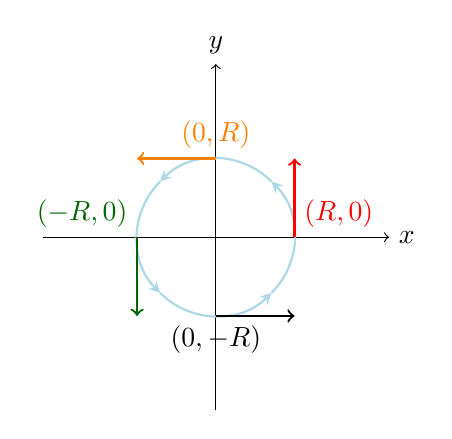
\begin{tikzpicture}
                \draw[->] (-2.2,0) -- (2.2,0) node[right] {$x$};
                \draw[->] (0,-2.2) -- (0,2.2) node[above] {$y$};
            
                \draw[thick,LightBlue,-stealth] (0.7071,0.7071) arc(45:135:1);
                \draw[thick,LightBlue,-stealth] (-0.7071,0.7071) arc(135:225:1);
                \draw[thick,LightBlue,-stealth] (-0.7071,-0.7071) arc(225:315:1);
                \draw[thick,LightBlue,-stealth] (0.7071,-0.7071) arc(-45:45:1);
            
                \node[red,above right] at (1,0) {$(R,0)$};
                \draw[thick,red,->] (1,0) -- (1,1);
                \node[orange,above] at (0,1) {$(0,R)$};
                \draw[thick,orange,->] (0,1) -- (-1,1);
                \node[DarkGreen,above left] at (-1,0) {$(-R,0)$};
                \draw[thick,DarkGreen,->] (-1,0) -- (-1,-1);
                \node[below] at (0,-1) {$(0,-R)$};
                \draw[thick,->] (0,-1) -- (1,-1);
            \end{tikzpicture}
        \end{center}
    \end{minipage}
\end{example}

When we need a parametrization of a curve, we typically choose the easiest one.

\subsection*{2D Parametrization}

$$f(u, v): \mathbb{R}^2 \to \mathbb{R}^3$$ where we have used the variables $u, v$ as the inputs of $f$. Thus for each $(u, v)$ in 2D, $f(u, v) = (x, y, z)$ is a point in 3D. 

Given a 2D region in the domain $\mathbb{R}^2$ (such as a square), $f(u, v)$ will create a surface in 3D. Since a surface is a 2D object, this is called a \term{2D parametrization}. 

\begin{itemize}
    \item Going from left to right, we may think that $f$ lifts up a 2D region in $\mathbb{R}^2$ into 3D, and maybe stretches the region somewhat, depending on the definition of $f$.
    
    \item Going from right to left, given a surface $S$ in 3D, we can try to find a parametrization for this surface $f(u, v) = (x, y, z)$. $f$ pulls back this (curved) surface $S$ in 3D with $(x, y, z)$ as variables, into a flat region in 2D with $(u, v)$ as variables.
\end{itemize}

We know that an equality involving $x$, $y$, $z$ gives a surface in 3D: $g(x, y, z) = 0$. This gives an alternative way of describing a surface in 3D. Finding a parametrization for a given surface is also an important skill in Calculus.

\begin{example}
    If we consider the plane $z = x + y + 10$ that is above the unit square on the $xy$-plane, we may choose the parametrization to be $$f(u, v) = (u, v, u + v + 10) = (x, y, z) \qquad u \in [0, 1] \qquad v \in [0, 1]$$

    This is called the natural parametrization, as we have set $u = x$ and $v = y$. For any point $(x, y) = (u, v)$ on the $xy$-plane, $f$ takes in this point, and gives out the same point with a new 3rd coordinate, or height, with the 3rd component defined by $f: z = u + v + 10$.

    This \itblue{lifts up} the unit square from the $xy$-plane, onto the plane $z = x + y + 10$. However, notice that the square is now slanted, and also stretched. In this case, the plane $z = x + y + 10$ is flat, but in general, $f$ lifts up a flat region in 2D, into a curved surface in 3D, with some stretching.
    
    \begin{minipage}{0.45\linewidth}
        \begin{center}
            \tikzsetnextfilename{c05s02-f02}%
            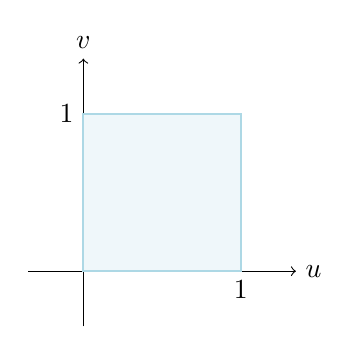
\begin{tikzpicture}
                \draw[->] (-0.7,0) -- (2.7,0) node[right] {$u$};
                \draw[->] (0,-0.7) -- (0,2.7) node[above] {$v$};

                \draw[thick,LightBlue,fill=LightBlue,fill opacity=0.2] (0,0) -- (0,2) -- (2,2) -- (2,0) -- cycle;

                \node[below] at(2,0) {$1$};
                \node[left] at(0,2) {$1$};
            \end{tikzpicture}
        \end{center}
    \end{minipage}
    \begin{minipage}{0.45\linewidth}
        \begin{center} 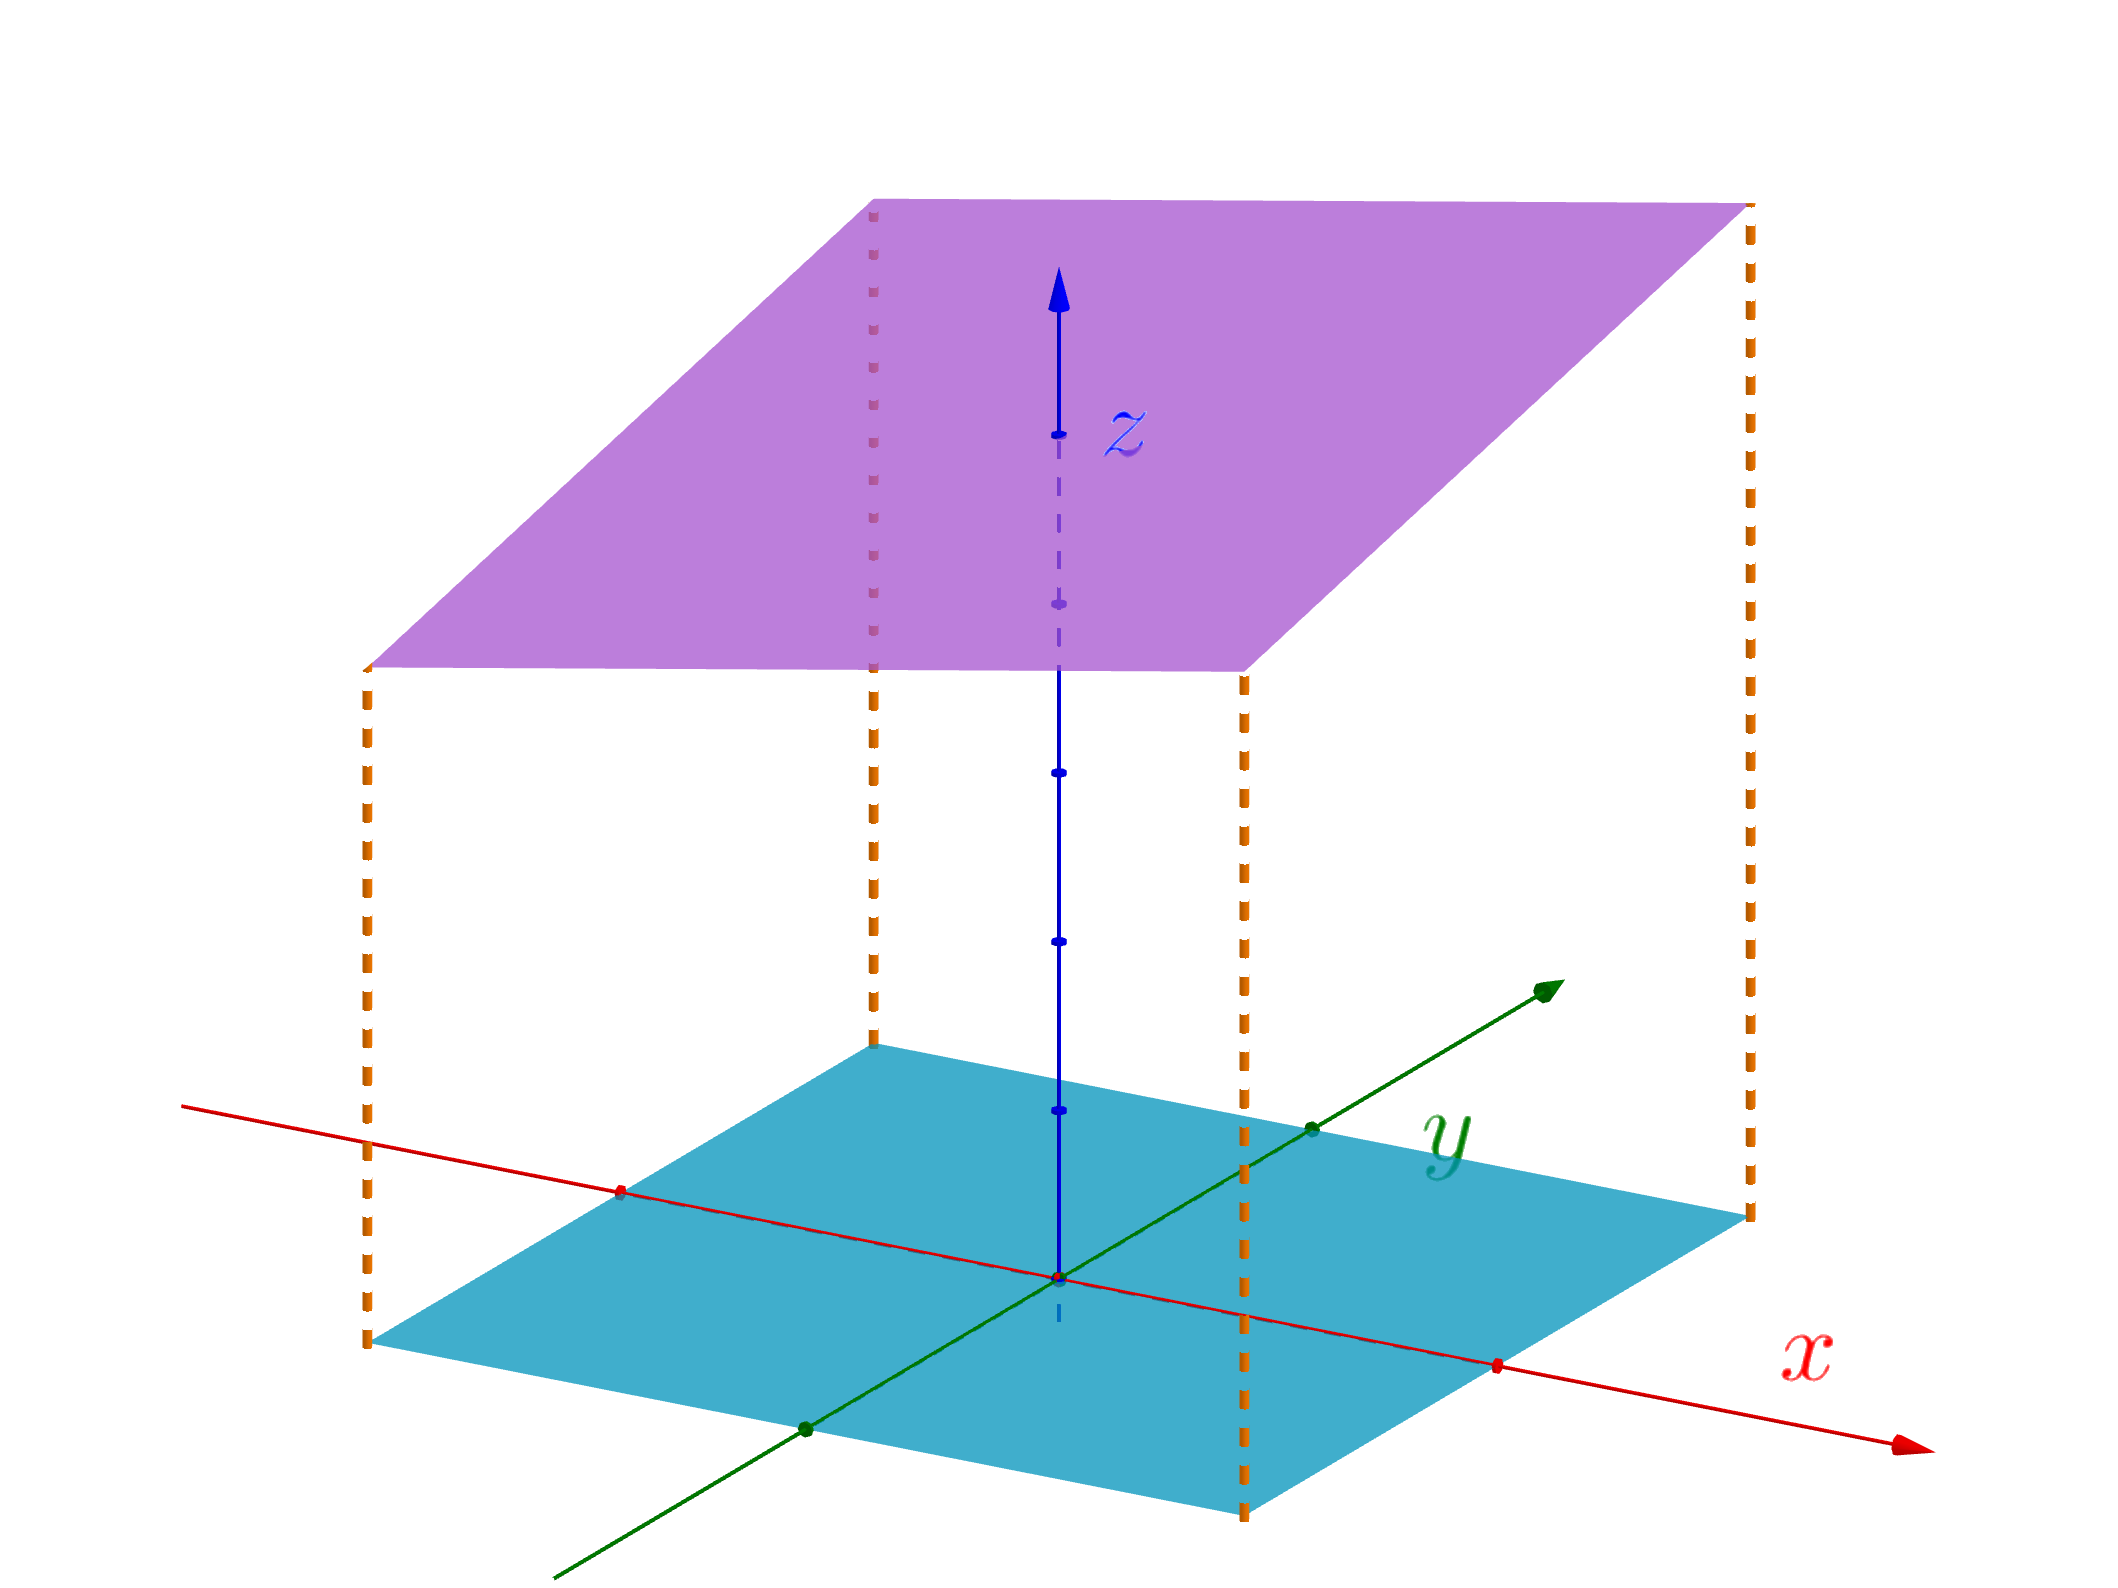
\includegraphics[width=0.95\linewidth]{Plots/s_5_2/u_v_uv10.png} \end{center}
    \end{minipage}

    In reverse, we can view $f$ pulls back a (possibly complicated) surface in 3D, (in this case $z = x + y + 10$), into a flat region in 2D (the unit square).
\end{example}

\section{Coordinate Transformation}

\begin{definition}[Coordinate Transformation]\index{Coordinate Transformation}
    When $f$ goes between spaces of the same dimension, we sometimes call $f$ a \term{coordinate transformation}. 

    $$f(u, v): \mathbb{R}^2 \to \mathbb{R}^2 \qquad \textbf{OR} \qquad f(u, v, w): \mathbb{R}^3 \to \mathbb{R}^3$$ where $f(u, v) = (x, y)$, and $f(u, v, w) = (x, y, z)$.
\end{definition}

\begin{itemize}
    \item Going from left to right, given a 2D region in the domain $\mathbb{R}^2$ (such as a square), $f(u, v) = (x, y)$ will produce another 2D region in $\mathbb{R}^2$, with some stretching as defined by $f$.

    \item Going from right to left, given a (possibly complicated) region in 2D with variables $(x, y)$, we can try to find a coordinate transformation $f$ for this region, where $f(u, v)$ transforms a simple region in the $uv$-plane, onto the original region in the $xy$-plane.
\end{itemize}

We have found a new set of coordinates $(u, v)$, to describe the more complicated region in the $xy$-plane.

Similarly, we can also do this for regions in 3D.

\begin{example}
    Given a \bred{solid} circle of radius $R$ at the origin, $x^2 + y^2 \le R^2$, it is a region in 2D. We know that representing this region is complicated in $(x, y)$, where we get expressions such as $y = \sqrt{R^2 - x^2}$.

    However, we may consider \term{polar coordinates}: $$f(r,\theta) = (r\cos{\theta},r\sin{\theta}) = (x,y) \qquad r \in [0,R] \qquad \theta \in [0,2\pi]$$ where for each point $(r,\theta)$ in the ``$r - \theta$'' plane, $f(r,\theta) = (x,y)$ is a point in the solid circle in the $xy$-plane.

    In other words, $f$ transforms a solid rectangle in the ``$r - \theta$'' plane, into the solid circle in the $xy$-plane. Instead of working with a circle, we now can work with a rectangle instead, as we have found \bred{better coordinates} to describe the original region in the $xy$-plane.
\end{example}

For $f$ to turn a rectangle into a circle, it must stretch the rectangle at multiple places, at different rates, which is based on the definition of $f$.

\section{Derivative Matrix}

Given a vector function, for example $f(x,y,z)$, $$f\begin{bmatrix} x \\ y \\ z \end{bmatrix} = \begin{bmatrix} f_1(x,y,z) \\ f_2(x,y,z) \\ f_3(x,y,z) \end{bmatrix}$$

The derivative of a vector function is $D_f$, called the derivative matrix.

For the first row of the matrix, we take the first coordinate function, and take the partial derivative with respect to all possible variables $(x,y,z)$ \bred{in order}, horizontally. Then for each coordinate function, we do the same thing to get a new row of the matrix. 

$$D_f = \begin{bmatrix}
    \frac{\partial}{\partial x} f_1 & \frac{\partial}{\partial y} f_1 & \frac{\partial}{\partial z} f_1 \\
    \frac{\partial}{\partial x} f_2 & \frac{\partial}{\partial y} f_2 & \frac{\partial}{\partial z} f_2 \\
    \frac{\partial}{\partial x} f_3 & \frac{\partial}{\partial y} f_3 & \frac{\partial}{\partial z} f_3 \\
\end{bmatrix}$$

\subsection*{Relation to Gradient $\nabla f$}

For a multi-variable function $f(x, y, z): \mathbb{R}^3 \to \mathbb{R}$, it returns one value (for example, $f(x,y,z) = xyz^2$). $$D_f = \nabla f = (\frac{\partial}{\partial x} f, \frac{\partial}{\partial y} f, \frac{\partial}{\partial z} f)$$ where the derivative matrix has only 1 row. 

On the other hand, for a vector function: $f(x, y, z) = (f_1, f_2, f_3)$, each row
of Df is the gradient of all the coordinate functions: $$D_f = \begin{bmatrix} - \nabla f_1 - \\ - \nabla f_2 - \\ - \nabla f_3 - \end{bmatrix}$$ where $\nabla f_i$ are viewed as horizontal vectors in the matrix.

\begin{exercise}
    $$f(x, y, z) = (3x + y, e^yz, xyz)$$

    First, state the dimension of the vector $f$ takes in, and the dimension of the vector $f$ gives out. Then, compute $D_f$.
\end{exercise}

\section{Change of Variable Formula}

Suppose you need to integrate $f$ over a domain $B$, but $B$ is very bad, You don't want to integrate over a bad domain. Suppose you can find a function $g$ such that $g$ takes another region a onto B. $$g: A \to B \qquad g(A) = B$$ and somehow $A$ is good domain. 

So, instead of integrating $f$ over the bad domain $B$, you can integrate over the good domain $A$ instead. $$\int_B f = \int_A f \circ g \cdot \left| \det(D_g) \right|$$ $f \circ g$ means replacing the old variables of $f$ in $B$ with the new ones in $A$ (we require that $g$ to be a one-to-one transformation, and $\det(D_g) \neq 0)$. The natural question is of course: How do I find such $g$?

\subsection*{1. Polar Coordinates}

Need to integrate $f(x, y)$. 

We take $g(r,\theta) = (r\cos{\theta},r\sin{\theta}) = (x,y)$. 

$f \circ g = f(g(r, \theta)) = f(r\cos{\theta}, r\sin{\theta}) = f(x, y)$ and $r^2 = x^2 + y^r$. 
$$\det(D_f) = r$$

This is useful when domain $B$ is (partly) of circular shape, or function given is already in polar coordinates.

\begin{minipage}{0.45\linewidth}
    \begin{center}
        \tikzsetnextfilename{c05s05-s01-f01-l}%
        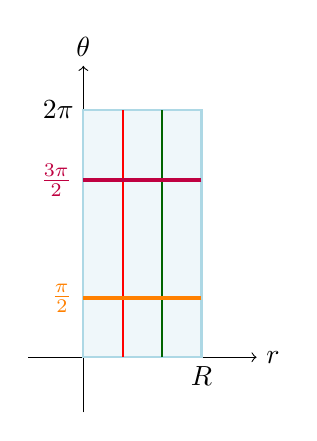
\begin{tikzpicture}
            \draw[->] (-0.7,0) -- (2.2,0) node[right] {$r$};
            \draw[->] (0,-0.7) -- (0,3.7) node[above] {$\theta$};
            
            \draw[thick,LightBlue,fill=LightBlue,fill opacity=0.2] (0,0) -- (0,3.14) -- (1.5,3.14) -- (1.5,0) -- cycle;
            \draw[thick,red] (0.5,0) -- (0.5,3.14);
            \draw[thick,DarkGreen] (1,0) -- (1,3.14);
            
            \draw[ultra thick,orange] (1.5,0.75) -- (0,0.75) node[left] {$\frac{\pi}{2}$};
            \draw[ultra thick,purple] (1.5,2.25) -- (0,2.25) node[left] {$\frac{3\pi}{2}$};
            
            \node[below] at(1.5,0) {$R$};
            \node[left] at(0,3.14) {$2\pi$};
        \end{tikzpicture}
    \end{center}
\end{minipage}
$\overset{g}{\longrightarrow}$
\begin{minipage}{0.45\linewidth}
    \begin{center}
        \tikzsetnextfilename{c05s05-s01-f01-r}%
        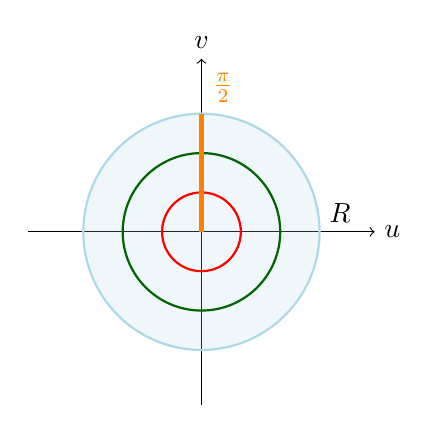
\begin{tikzpicture}
            \draw[->] (-2.2,0) -- (2.2,0) node[right] {$u$};
            \draw[->] (0,-2.2) -- (0,2.2) node[above] {$v$};
            
            \draw[thick,LightBlue,fill=LightBlue,fill opacity=0.2] (0,0) circle(1.5);
            \draw[thick,red] (0,0) circle(0.5);
            \draw[thick, DarkGreen] (0,0) circle(1);
            
            \draw[ultra thick,orange] (0,0) -- (0,1.5) node[above right] {$\frac{\pi}{2}$};
            
            \node[above right] at(1.5,0) {$R$};
        \end{tikzpicture}
    \end{center}
\end{minipage}

\begin{exercise}
    Integrate $f(x,y) = x$ over $D = {1 \le x^2 + y^2 \le 4}$ in the 2nd quadrant.
\end{exercise}

\begin{exercise}
    Show that $\int_{-\infty}^{+\infty} e^{-x^2} \,dx = \sqrt{\pi}$

    \textbf{Strategy: } The normal distribution has no anti-derivative. Start with $\left( \int_{-\infty}^{+\infty} e^{-x^2} \right)^2$ and write it as a product of 2 same things. Then change the variable in one integral from $x$ to $y$, and use the polar coordinate transformation.
\end{exercise}

\subsubsection*{Polar Curves}

$r$ represent the distance from the point $(x, y)$ to the origin, $\theta$ represent the angle rotated counterclockwise from $x$-axis to the point. Negative angles represent angles rotated clockwise. Thus $\theta = \pi$ is the same as $\theta = -\pi$.

If $r$ is negative, it represent the point on the line with angle $\theta$ through the origin, except on the opposite side of the line, with radius being $|r|$.

\begin{center}
   \tikzsetnextfilename{c05s05-s01-f02}%
    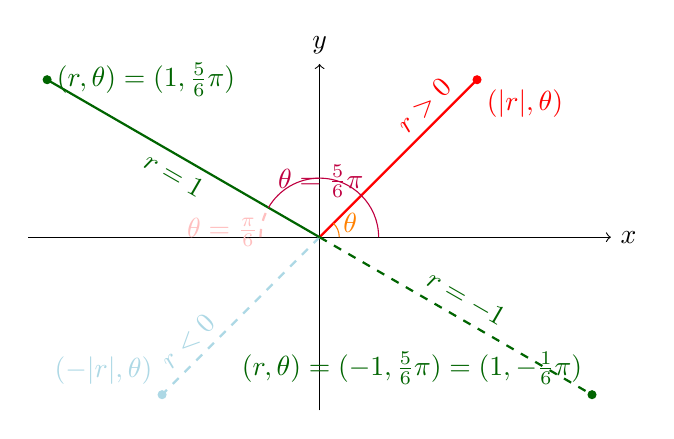
\begin{tikzpicture}
        \draw[->] (-3.7,0) -- (3.7,0) node[right] {$x$};
        \draw[->] (0,-2.2) -- (0,2.2) node[above] {$y$};
        
        \draw[thick,red] (2,2) -- (0,0);
        \draw[thick,LightBlue,dashed] (0,0) -- (-2,-2);
        \draw[orange] (0.25,0) arc(0:45:0.25) node[right] {$\theta$};
        
        \draw[thick,DarkGreen] (-3.46,2) -- (0,0);
        \draw[thick,DarkGreen,dashed] (0,0) -- (3.46,-2);
        \draw[purple] (0.75,0) arc(0:150:0.75) node[above right] {$\theta=\frac{5}{6}\pi$};
        \draw[thick,pink,dashed] (-0.75,0) arc(180:150:0.75) node[below left] {$\theta=\frac{\pi}{6}$};
        
        \draw[red,fill=red] (2,2) circle(0.05) node[below right] {$(|r|, \theta)$};
        \draw[LightBlue,fill=LightBlue] (-2,-2) circle(0.05) node[above left] {$(-|r|, \theta)$};
        \draw[DarkGreen,fill=DarkGreen] (-3.46,2) circle(0.05) node[right] {$(r,\theta) = (1,\frac{5}{6}\pi)$};
        \draw[DarkGreen,fill=DarkGreen] (3.46,-2) circle(0.05) node[above left] {$(r,\theta) = (-1,\frac{5}{6}\pi) = (1, -\frac{1}{6}\pi)$};
        
        \node[red,above,rotate=45] at (1.5,1.5) {$r>0$};
        \node[LightBlue,above,rotate=45] at (-1.5,-1.5) {$r<0$};
        \node[DarkGreen,below,rotate=-30] at (-1.73,1) {$r=1$};
        \node[DarkGreen,above,rotate=-30] at (1.73,-1) {$r=-1$};
    \end{tikzpicture}
\end{center}

\begin{example}
    The point $(r, \theta) = (1, \frac{3\pi}{4})$ in the polar coordinates represent $(x, y) = (-\frac{1}{\sqrt{2}}, \frac{1}{\sqrt{2}})$. 

    The point $(r, \theta) = (-1, \frac{3\pi}{4})$ in the polar coordinates has $r$ as negative. We go on the line $\frac{3\pi}{4}$, which is toward the top left. Since $r$ is negative, we go on the opposite side of the line, and take the point with radius being $|r| = 1$. Thus $(-1, \frac{3\pi}{4})$ in the polar coordinates represent $(x, y) = (\frac{1}{\sqrt{2}}, -\frac{1}{\sqrt{2}})$. 
\end{example}

Using the above convention, we can define polar curve: $r = h(\theta)$. To draw the polar curve, we pick some values of $\theta$, and plot the value of $r$ specified by $r = h(\theta)$ on the line represented by $\theta$.

\begin{itemize}
    \item $r = a$ gives the circle with radius $a$ centered at the origin.

    \begin{center}
        \tikzsetnextfilename{c05s05-s01-f03-01}%
        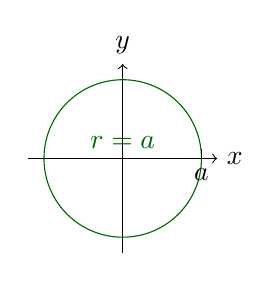
\begin{tikzpicture}
            \draw[->] (-1.2,0) -- (1.2,0) node[right] {$x$};
            \draw[->] (0,-1.2) -- (0,1.2) node[above] {$y$};
            
            \draw[DarkGreen] (0,0) circle(1.0) node[above] {$r=a$};
            
            \draw (1.0,0.125) -- (1.0,0) node[below] {$a$};
        \end{tikzpicture}
    \end{center}

    \item $r = a\cos{\theta}$ gives the circle to the right (if $a > 0$).
    
    The circle is between the points $(a, 0)$ and the origin. The radius is $\frac{a}{2}$.

    $\begin{aligned}[t]
        r                                                                        & = a \cos{\theta}             \\
        r^2                                                                      & = r a \cos{\theta}           \\
        x^2 + y^2                                                                & = ax                         \\
        x^2 - ax + \left(\frac{a}{2}\right)^2 + y^2 - \left(\frac{a}{2}\right)^2 & = 0                          \\
        \left(x - \frac{a}{2}\right)^2 + y^2                                     & = \left(\frac{1}{2}\right)^2
    \end{aligned}$

    \begin{center}
        \tikzsetnextfilename{c05s05-s01-f03-02}%
        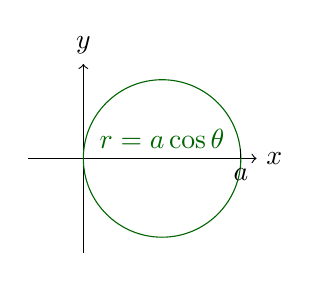
\begin{tikzpicture}
            \draw[->] (-0.7,0) -- (2.2,0) node[right] {$x$};
            \draw[->] (0,-1.2) -- (0,1.2) node[above] {$y$};
            
            \draw[DarkGreen] (1,0) circle(1.0) node[above] {$r=a\cos{\theta}$};
            
            \draw (2,0.125) -- (2,0) node[below] {$a$};
        \end{tikzpicture}
    \end{center}

    \begin{minipage}{0.36\linewidth}
        \begin{center}
            \tikzsetnextfilename{c05s05-s01-f03-02-l}%
            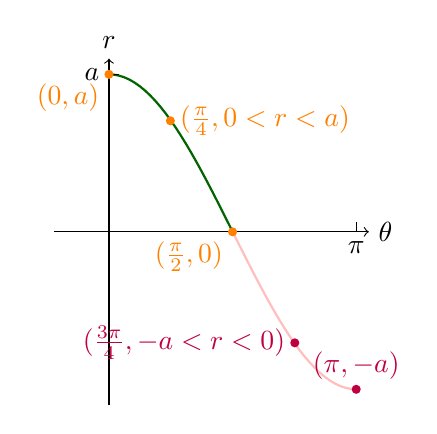
\begin{tikzpicture}
                \draw[->] (-0.7,0) -- (3.3,0) node[right] {$\theta$};
                \draw[->] (0,-2.2) -- (0,2.2) node[above] {$r$};

                \draw[thick,DarkGreen,domain=0:1.57] plot(\x, {2*cos(deg(\x))});
                \draw[thick,pink,domain=1.57:3.14] plot(\x, {2*cos(deg(\x))});

                \draw (3.14,0.125) -- (3.14,0) node[below] {$\pi$};
                \draw (0.125,2) -- (0,2) node[left] {$a$};

                \draw[orange,fill=orange] (0,2) circle(0.05) node[below left] {$(0,a)$};
                \draw[orange,fill=orange] (0.78,1.41) circle(0.05) node[right] {$(\frac{\pi}{4},0<r<a)$};
                \draw[orange,fill=orange] (1.57,0) circle(0.05) node[below left] {$(\frac{\pi}{2},0)$};

                \draw[purple,fill=purple] (2.36,-1.41) circle(0.05) node[left] {$(\frac{3\pi}{4},-a<r<0)$};
                \draw[purple,fill=purple] (3.14,-2) circle(0.05) node[above] {$(\pi,-a)$};
            \end{tikzpicture}
        \end{center}
    \end{minipage}
    \begin{minipage}{0.63\linewidth}
        \begin{center}
            \tikzsetnextfilename{c05s05-s01-f03-02-r}%
            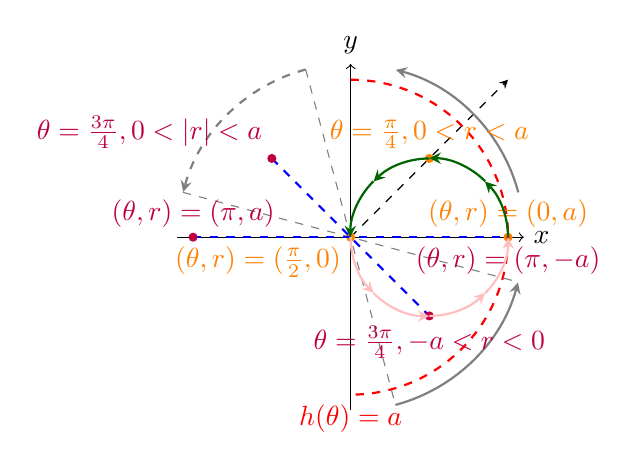
\begin{tikzpicture}
                \draw[->] (-2.2,0) -- (2.2,0) node[right] {$x$};
                \draw[->] (0,-2.2) -- (0,2.2) node[above] {$y$};

                \draw[dashed,-stealth] (0,0) -- (2,2);

                \draw[thick,red,dashed] (0,2) arc(90:-90:2) node[below] {$h(\theta)=a$};
                \draw[thick,gray,-stealth] (2.13,0.57) arc(15:75:2.2);
                \draw[thick,gray,-stealth,dashed] (-0.57,2.13) arc(105:165:2.2);
                \draw[thick,gray,-stealth] (0.57,-2.13) arc(285:345:2.2);
                \draw[gray,dashed] (-0.57,2.13) -- (0.57,-2.13);
                \draw[gray,dashed] (-2.13,0.57) -- (2.13,-0.57);

                %
                \draw[orange,fill=orange] (2,0) circle(0.05) node[above] {$(\theta,r)=(0,a)$};
                \draw[orange,fill=orange] (1,1) circle(0.05) node[above] {$\theta=\frac{\pi}{4},0<r<a$};
                \draw[orange,fill=orange] (0,0) circle(0.05) node[below left] {$(\theta,r)=(\frac{\pi}{2},0)$};

                \draw[thick,blue,dashed] (-2,0) -- (2,0);
                \draw[purple,fill=purple] (-2,0) circle(0.05) node[above] {$(\theta,r)=(\pi,a)$};
                \draw[purple,fill=purple] (2,0) circle(0.0125) node[below] {$(\theta,r)=(\pi,-a)$};

                \draw[thick,blue,dashed] (-1,1) -- (1,-1);
                \draw[purple,fill=purple] (-1,1) circle(0.05) node[above left] {$\theta=\frac{3\pi}{4},0<|r|<a$};
                \draw[purple,fill=purple] (1,-1) circle(0.05) node[below] {$\theta=\frac{3\pi}{4},-a<r<0$};

                %
                \draw[thick,DarkGreen,-stealth] (2,0) arc(0:45:1);
                \draw[thick,DarkGreen,-stealth] (1.71,0.71) arc(45:90:1);
                \draw[thick,DarkGreen,-stealth] (1,1) arc(90:135:1);
                \draw[thick,DarkGreen,-stealth] (0.29,0.71) arc(135:180:1);
                \draw[thick,pink,-stealth] (0,0) arc(180:225:1);
                \draw[thick,pink,-stealth] (0.29,-0.71,0) arc(225:270:1);
                \draw[thick,pink,-stealth] (1,-1) arc(270:315:1);
                \draw[thick,pink,-stealth] (1.71,-0.71) arc(315:360:1);
            \end{tikzpicture}
        \end{center}
    \end{minipage}

    \item $r = b\sin{\theta}$ gives the circle to the top (if $b > 0$).

    The circle is between the points $(0, b)$ and the origin. The radius is $\frac{b}{2}$.
    \begin{center}
        \tikzsetnextfilename{c05s05-s01-f03-03}%
        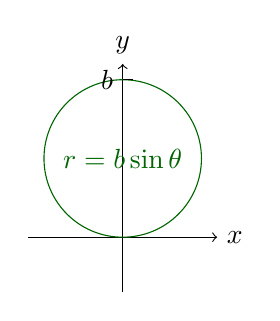
\begin{tikzpicture}
            \draw[->] (-1.2,0) -- (1.2,0) node[right] {$x$};
            \draw[->] (0,-0.7) -- (0,2.2) node[above] {$y$};
            
            \draw[DarkGreen] (0,1) circle(1.0) node {$r=b\sin{\theta}$};
            
            \draw (0.125,2) -- (0,2) node[left] {$b$};
        \end{tikzpicture}
    \end{center}
\end{itemize}

\begin{exercise}
$\text{ }$

    \begin{enumerate}[label=\alph*)]
        \item Find the area enclosed by polar curve $h(\theta)$, but outside of polar curve $k(\theta)$: $h(\theta) = r = 1 + \cos(\theta)$, $k(\theta) = r = 3\cos(\theta)$. 

        \textbf{Strategy: } plot the curve. Find the intersection between the polar curves. First choose the min and max value of $\theta$ as the outer integral, then $r$ would start from the smaller value (inner polar curve) to the larger value (outer polar curve).

        \item Sketch the curve $r = 1 + 2\cos{\theta}$ and find the area it encloses in the outer loop but outside the inner loop.

        \textbf{Strategy: } this shape is complicated and it crosses itself. We can not apply the formula directly , we need to use symmetry and subtract the inner area.
    \end{enumerate}
\end{exercise}

\subsection*{2. Cylindrical Coordinates}

We need to integrate $f(x, y, z)$. Take $g(r, \theta, z) = (r\cos(\theta), r\sin(\theta), z) = (x,y,z)$. 

For any specific point $(x, y, z)$, it can be described as a radius, a height and an angle:

\begin{center}
    %TODO: finish graph
    \begin{tikzpicture}
        \draw[->] (0,0) -- (2.2,0) node[right] {$y$};
        \draw[->] (0,0) -- (0,2.2) node[above] {$z$};
        \draw[->] (0,0) -- (-1.41,-1.41) node[below left] {$x$};

        \draw[dashed] (-0.71, -0.71) -- (0.29,-0.71);
        \draw[dashed] (0.29, -0.71) -- (1,0);
        \draw[dashed] (0.29, -0.71) -- (0.29,0.29);
        \draw[dashed] (0.29,0.29) -- (0,1);
        \draw[dashed] (0.29,-0.71) -- (0,0);
    \end{tikzpicture}
\end{center}

\begin{itemize}
    \item $r$ is the distance between the point and the \bred{$z$-axis};
    \item $\theta$ is the angle between the $x$-axis and the point $(x,y,0)$ \footnote{$(x,y,0)$ is the projection of the point onto the $xy$-plane. };
    \item $z$ is the height.
\end{itemize}

$f \circ g = f(g(r, \theta, z)) = f(r\cos(\theta), r\sin(\theta), z)$ and $r^2 = x^2 + y^2$. 
$$\det(D_g) = r$$

This is useful when 
\begin{itemize}
    \item domain $B$ is partly of cylindrical shape or has circular projection, or
    \item function given is already in cylindrical coordinates, or
    \item the domain can be obtained through a rotation with the defining equations containing $x^2 + y^2$.
\end{itemize}

\textbf{Graphing Surfaces attained through rotation}

When the variables $x$ and $y$ in the defining equations can be written \bred{completely} with $r^2 = x^2 + y^2$, this signals that the surface is attained through rotation. We graph the 2D curves involving $z$ and $r$ in the $rz$-plane. We revolve the curves around the $z$-acis to attain surfaces in 3D. To integrate the volume bounded by the surfaces, we need to use cylindrical coordinates and preform a \bred{2D integration} in the $rz$-plane, and then we add the $\theta$-integral to the outside. \bred{Don't forget to include the term $\det(D_g) = r$}. We only integrate the portion with $r > 0$. 

\begin{exercise}
    $z = h(x,y) = a \cdot \left( \sqrt{x^2 + y^2} - 1 \right)^2$, with $a > 0$. 

    Consider the volume inside the cylinder $x^2 + y^2 = 1$, above $z = 0$, and below $z = h(x,y)$. 

    Find $a$ so that the volume is $1$. 
\end{exercise}

\subsection*{3. Spherical Coordinates}

We need to integrate $f(x, y, z)$. Take $g(\rho, \phi, \theta) = (\rho \sin(\phi) \cos(\theta), \rho \sin(\phi) \sin(\theta), \rho\cos(\phi)) = (x, y, z)$

For any specific point $(x, y, z)$, it can be described by the radius and the 2 angles: 

% TODO: add graph

\begin{itemize}
    \item $\rho$ is the distance from the point to the \bred{origin}, as the radius;
    \item $\phi$ is the angle between the $z$-acis and the point $(x, y, z)$ \footnote{This is called \term{inclination angle}. };
    \item $\theta$ is the angle between the $x$-axis and the point onto the $xy$-plane \footnote{This is called \term{azimuthal angle}. }.
\end{itemize}

Note that $r$ and $\rho$ both represents `radius' in Spherical and Cylindrical Coordinates, but they stand for \bred{different radii}. 

$f \circ g = f(g(\rho, \theta, \phi)) = f(\rho \sin(\phi) \cos(\theta), \rho \sin(\phi) \sin(\theta), \rho \cos(\phi)) = f(x, y, z)$, and $\rho^2 = x^2 + y^2 + z^2$. 
$$\det(D_g) = \rho^2 \sin(\phi)$$

This is useful when the domain $B$ is (partly) of spherical shaper, or function given is already in spherical coordinates. 

The maximum value of $\phi$ is $\pi$ (180$^\circ$), at most to the negative $z$-axis. For a full sphere of radius $R$, the range of the variables are 
\begin{itemize}
    \item $\rho: 0 \to R$
    \item $\phi: 0 \to \pi$
    \item $\theta: 0 \to 2\pi$
\end{itemize}

If the sphere is \bred{not} centred at the origin, spherical coordinates is usually \bred{not} the choice. 

\begin{exercise}
    Find the 3D-volume of a solid hemisphere in $\mathbb{R}^3$ with radius $R$ and $x > 0$. 

    \textbf{Strategy}: recall integrating the function $f = 1$ gives the volume of the domain. 
\end{exercise}

\begin{exercise}
    Consider the surface $A$ characterized by $z = \sqrt{3} \sqrt{(x^2 + y^2)} = \sqrt{3} \cdot r$, where $r$ is the radius in \textbf{cylindrical coordinates}. Consider the surface $B$ as the sphere of radius $2$, $x^2 + y^2 + z^2 = 4$. Find the volume bounded by surface $A$ and $B$ in 2 ways:

    \begin{enumerate}[label=\alph*)]
        \item Use Spherical Coordinates.
        
        \textbf{Strategy}: Plot the curve in the $rz$-plane, and rotate to a 3D volume. The volume looks like an ice-cream cone. What is the maximum inclination angle $\phi$? Remember that $r$ in both coordinates are not the same.

        \item Use Cylindrical Coordinates. Which method do you think is more suited?
        
        \textbf{Strategy}: Solve the intersection of the surfaces by plugging a quantity of one equation into the other. Perform a 2D integral in $rz$-plane, and add the $\theta$-integral on the outside.
        
        \item Now consider surface $C$ as the plane $z = \sqrt{3}$. What is the volume between surface $A$ and $C$? Which method should you use?
    \end{enumerate}
\end{exercise}

\begin{exercise}
    Compute the volume above the cone $z = \sqrt{x^2 + y^2}$ and below the sphere $x^2 + y^2 + z^2 = 2z$. 

    \begin{enumerate}[label=\alph*)]
        \item Use Cylindrical Coordinates.
        
        \textbf{Strategy}: Why is it a sphere? Plot the curve on the $rz$-plane. For the sphere, complete the square in $z$. Find the intersection and perform a 2D integral in $rz$-plane.

        \item Use Spherical Coordinates. Which way do you prefer?
        
        \textbf{Strategy}: Since the sphere is \bred{not} centered at the origin, the range of $\rho$ is \bred{not} $0$ to $1$. Use the defining equation $x^2 + y^2 + z^2 = 2z$ and switch variables to spherical coordinates to attain $\rho = 2\cos(\phi)$. Notice $\rho$ varies in terms of the value $\phi$ in 3D, similar to polar curves in 2D, so we \bred{must} put it as the innermost integral.
    \end{enumerate}
\end{exercise}

\subsection*{Ellipse Transformation}

To integrate over an ellipse, we write the equation of ellipse as $\left(\frac{x}{a}\right)^2 + \left(\frac{y}{b}\right)^2 = 1$.

Similar to polar coordinates, we use $g(r, \theta) = (a \cdot r \cos{\theta}, b \cdot r \sin{\theta})$. Note that $\det(D_h) = abr$. 

Since the stretching factors of the ellipse are included in function $g$, the range of radius is \bred{always} $r: 0 \to 1$.

$\theta$ does not exactly represent the angle from polar coordinates anymore, though it still works as normal for these angles, $\theta = 0, \frac{\pi}{2}, \pi, \frac{3\pi}{2}, 2\pi, \dots$. A full ellipse is still $\theta: 0 \to 2\pi$. 

This is useful when a 2D domain is an ellipse, or if the 3D projection of a volume is of ellipse shape.

\begin{exercise}
   Verify $\det(D_g) = abr$, Then find the area of the ellipse given by the standard equation above.
\end{exercise}

\begin{exercise}
    Integrate $f(x, y) = \sin(2x^2 + 4y^2)$ over the region bounded by $2x^2 + 4y^2 = 4$.
\end{exercise}

\begin{exercise}
    Compute the volume above $z = \sqrt{2x^2 + y^2}$ and below $z = 2$. 

    \textbf{Strategy}: This surface is not given by a circular rotation, with $r^2 = x^2 + y^2$. However, it is similar. We may take the ``radius'' to be $r^2 = 2x^2 + y^2$, so we can still plot on the $rz$-plane and do an ellipse rotation. Taking the projection of the volume onto the $xy$-plane gives an ellipse. Instead of integrating the 2D projection integral directly, we first perform the inner $z$-integral, and use ellipse transformation onto the 2D integral.
\end{exercise}

\subsection*{Parallelogram Transformation}

Given a parallelogram in $\mathbb{R}^2$ with one vertex being origin. It is generated by 2 points/vectors, $\vec{a}$ and $\vec{b}$. We can turn the unit square into parallelogram by requiring that $$g\begin{bmatrix} 1 \\ 0 \end{bmatrix} = \vec{a} \qquad g\begin{bmatrix} 0 \\ 1 \end{bmatrix} = \vec{b}$$ Since the parallelogram is linear, this is a linear transformation. It is characterized by a matrix. $$g\begin{bmatrix} u \\ v \end{bmatrix} = A \cdot \begin{bmatrix} u \\ v \end{bmatrix} = \begin{bmatrix} x \\ y \end{bmatrix}$$ Cue to the constraint on the unit vectors above, $A$ must be $$A = \begin{bmatrix} | & | \\ \vec{a} & \vec{b} \\ | & | \end{bmatrix}$$

If the parallelogram does not have one vertex at origin, we can perform a shift of the parallelogram, by subtracting the coordinates of one point from all points of the parallelogram. We take note of $\vec{a}$ and $\vec{b}$ that generate the \bred{shifted} parallelogram. The transformation g would take 2 steps. First the transformation of the square to the shifted parallelogram, then from the shifted parallelogram to the original one.

\begin{example}
    Given the parallelogram $(1, 1)$, $(2, 1)$, $(2, 2)$, $(3, 2)$ which is a standard $45$ degrees parallelogram that is shifted \footnote{The standard 45 degrees parallelogram is defined by the vectors $\begin{bmatrix} 1 \\ 0 \end{bmatrix}$ and $\begin{bmatrix} 1 \\ 1 \end{bmatrix}$. }. We can use the above transformation, to turn the unit square into the standard parallelogram using $$h\begin{bmatrix} u \\ v \end{bmatrix} = \begin{bmatrix} 1 & 1 \\ 0 & 1 \end{bmatrix} \cdot \begin{bmatrix} u \\ v \end{bmatrix}$$  We then need to shift the parallelogram upward and right by 1 unit. Thus $$g\begin{bmatrix} u \\ v \end{bmatrix} = \begin{bmatrix} 1 & 1 \\ 0 & 1 \end{bmatrix} \cdot \begin{bmatrix} u \\ v \end{bmatrix} + \begin{bmatrix} 1 \\ 1 \end{bmatrix}$$ In both the shifted and the non-shifted case, $D_g = A$. 
\end{example}

\subsection*{Tetrahedron Transformation}

Generalizing the idea of parallelogram, the tetrahedron transformation is much more useful in practice.

Given a tetrahedron in $\mathbb{R}^3$ with one vertex being the origin, it is characterized by 3 points/vectors, $\vec{a}$, $\vec{b}$, $\vec{c}$. We can turn the \itblue{unit tetrahedron} into the tetrahedron given by requiring that $$ g\begin{bmatrix} 1 \\ 0 \\ 0 \end{bmatrix} = \vec{a} \qquad g \begin{bmatrix} 0 \\ 1 \\ 0 \end{bmatrix} = \vec{b} \qquad g \begin{bmatrix} 0 \\ 0 \\ 1 \end{bmatrix} = \vec{c}$$ If we define the names of the variables of $g$ as $g(u, v, w)$, then our domain of integration is the unit tetrahedron, given by $$\int_{w=0}^{w=1} \int_{v=0}^{v=1-w}\int_{u=0}^{u=1-w-b} f \circ g  \cdot |\det(D_g)| \,du \,dv \,dw$$ Of course, $g$ is again a linear transformation, $$g \begin{bmatrix} u \\ v \\ w \end{bmatrix} = A \cdot \begin{bmatrix} u \\ v \\ w \end{bmatrix} = \begin{bmatrix} x \\ y \\ z \end{bmatrix}$$ where the matrix $A$, by the constraints above, is $$A = \begin{bmatrix} | & | & | \\ \vec{a} & \vec{b} & \vec{c} \\ | & | & | \end{bmatrix}$$ If the tetrahedron does not have one vertex at origin, we perform a shift similar to parallelogram. Same as the parallelogram transformation, in both the non-shifted and the shifted case, $D_g = A$. 

\begin{exercise}
    Find the volume bounded by $x + 2y + z = 2$, $x = 2y$, $x = 0$, $z = 0$.

    \textbf{Strategy}: Take any 3 planes, they intersect at 1 point. 4 points form a tetrahedron. 
\end{exercise}

\begin{exercise}
    Compute the integral $\int_D z - x - y$ where $D$ is the tetrahedron given by $D$ $(0,0,0)$, $(1,2,3)$, $(0,2,2)$, and $(-1,1,1)$.
\end{exercise}

\subsection*{Domain Bounded by 2 Expressions}

Sometimes, a 2D domain $B$ is defined by the region bounded by some curves given by $f_1(x,y) = a$, $f_1(x,y) = b$, $f_2(x,y) = c$, and $f_2(x,y) = d$. If the curves only intersect at 4 points, we can transform the square onto the domain by using $$h\begin{bmatrix} x \\ y \end{bmatrix} = \begin{bmatrix} f_1(x,y) \\ f_2(x,y) \end{bmatrix} = \begin{bmatrix} u \\ v \end{bmatrix}$$ and since $u = f_1(x,y)$ and $v = f_2(x,y)$, the bounds of $\begin{bmatrix} u \\ v \end{bmatrix}$ is exactly the square $A = \{ u \in (a, b)m v \in (c, d) \}$. 

However, computing inverse is sometimes difficult. Since we need $\det(D_g)$ in the formula, and $g = h^{-1}$, we can instead use $$\det(D_g) = \det(D_{h^{-1}}) = \det(\left(D_h\right)^{-1}) = \det(D_h)^{-1} = \frac{1}{\det(D_h)}$$ Thus we can simply compute $D_h$ which is given, and use it in the change of variable formula without needing to compute the inverse \footnote{ Note we may still need to compute the inverse sometimes. }. 

\begin{example}
    Integrate $f(x,y) = y$ over the domain $B$ given by $xy = 1$, $xy = 2$, $xy^2 = 1$, $xy^2 = 2$. 
    
    Set $u = xy$, $v = xy^2$. $D_h = \begin{bmatrix} y & x \\ y^2 & 2xy \end{bmatrix} \implies \det(D_h) = 2xy^2 - xy^2 = xy^2 = v$, so $\det(D_g) = \det(D_h)^{-1} = \frac{1}{v}$

    $\begin{aligned}[t]
        f(x, y) = y = \frac{v}{u} \implies \int_B y \,dA
         & = \int_A \frac{v}{u} \cdot \frac{1}{v} \,dA                \\
         & = \int_{u=1}^{u=2} \int_{v=1}^{v=2} \frac{1}{u}  \,dv \,du \\
    \end{aligned}$
\end{example}

\begin{exercise}
$\text{ }$

    \begin{enumerate}
        \item $\int_D(x+y)(x-y)$ over $D$ bounded by $x - y = 0$, $x - y = 2$, $x + y = 1$, $x + y = 2$. 
        \item $\int_D \sin\left( \frac{2x-y}{2x+y} \right)$ over $D$ bounded by $x = 0$, $y = 0$, $2x + y = 1$. 
    \end{enumerate}
\end{exercise}